\documentclass[12pt]{article}
% Full article preamble (duplicated, no common file)
\usepackage{fontspec}
\usepackage[a4paper,margin=2.5cm,includefoot]{geometry}
\usepackage{polyglossia}
\usepackage{amsmath}
\usepackage{amssymb}
\usepackage{xcolor}
\usepackage{fancyhdr}
\usepackage{graphicx}
\usepackage{listings}
\usepackage[most]{tcolorbox}
\usepackage{pifont}
\usepackage{enumitem}
\usepackage{titlesec}
\usepackage[bottom]{footmisc}
\usepackage{titling}
\usepackage{minted}
\usepackage{etoolbox}
\usepackage{array}
\usepackage{extsizes}

\newfontfamily\emoji{Segoe UI Emoji}

\pagestyle{fancy}

\setmainlanguage[numerals=western]{arabic}
\setotherlanguage{english}
\newfontfamily\arabicfont[Script=Arabic]{Amiri}
\newfontfamily\arabicfonttt[Script=Arabic]{Courier New}

\lstset{
  language=[Sharp]C,
  numbers=left,
  stepnumber=1,
  numbersep=8pt,
  frame=single,
  basicstyle=\ttfamily\small,
  keywordstyle=\color{blue},
  stringstyle=\color{red},
  commentstyle=\color{green!50!black}
}

\newif\ifdetailed
\ifdefined\setdetailed
  \setdetailed
\fi

\newif\ifwithsols
\ifdefined\setwithsols
  \setwithsols
\fi

% unified tcolorboxes for articles
\tcbset{colback=white, colframe=black, fonttitle=\bfseries, boxrule=0.8pt}
\newtcolorbox{boxDef}[1][]{colback=blue!5!white,colframe=blue!75!black,
  title={{\emoji📘} تعريف\ifx\\#1\\\else ~#1\fi :}}
\newtcolorbox{boxExercise}[1][]{colback=cyan!5!white,colframe=cyan!70!black,
  title={{\emoji🧩} تمرين\ifx\\#1\\\else ~#1\fi :}}
\newtcolorbox{boxExample}[1][]{colback=yellow!5!white,colframe=orange!90!black,
  title={{\emoji📝} مثال\ifx\\#1\\\else ~#1\fi :}}
\newtcolorbox{boxNote}[1][]{colback=gray!10!white,colframe=black,
  title={{\emoji✨} ملاحظة\ifx\\#1\\\else ~#1\fi :}}
\newtcolorbox{boxAttention}[1][]{colback=magenta!10!white,colframe=magenta!80!black,
  title={{\emoji🔔} تنبيه\ifx\\#1\\\else ~#1\fi :}}
\newtcolorbox{boxWarning}[1][]{colback=red!5!white,colframe=red!75!black,
  title={{\emoji⚡} ملاحظة هامة\ifx\\#1\\\else ~#1\fi :}}
\newtcolorbox{boxSolution}[1][]{colback=green!5!white,colframe=green!60!black,
  title={{\emoji✅} حل\ifx\\#1\\\else ~#1\fi :}}
\newtcolorbox{boxSymbol}[1][]{colback=purple!5!white,colframe=purple!70!black,
  title={{\emoji🔣} رمز\ifx\\#1\\\else ~#1\fi :}}

\tcbset{simplecode/.style={ colback=gray!5, colframe=black!50, boxrule=0.4pt, arc=2pt, left=4pt,right=4pt,top=4pt,bottom=4pt}}
\newenvironment{boxCode}{\begin{tcolorbox}[simplecode]}{\end{tcolorbox}}

\newcolumntype{C}[1]{>{\centering\arraybackslash}p{#1}}

% redefine spaces after titles
\makeatletter
\renewcommand{\@maketitle}{%
  \begin{center}
    {\huge \bfseries \@title \par}%
    \vskip 0.2em % space between title and author
    {\large \@author \par}%
    % \vskip 0.2em % space between author and date
    % {\normalsize \@date \par}%
  \end{center}
}
\makeatother

\fancyhf{} % clear default
\fancypagestyle{plain}{
  \fancyhf{}
  \fancyhead[L]{مدرسة التسامح الشاملة}
  % \fancyhead[L]{
\includegraphics[height=1cm]{../../../images/logoTasamoh.png}}
  \fancyhead[R]{الأستاذ محمود اغبارية}
  \fancyfoot[C]{\thepage}
}

\fancyhead[L]{مدرسة التسامح الشاملة}
\fancyhead[R]{الأستاذ محمود اغبارية}
\fancyfoot[C]{\thepage}
% \date{\today}

\setcounter{tocdepth}{3} % only section subsection and subsubsection in TOC


% ----------------------


% \begin{document}

% \maketitle

% % \clearpage  % start TOC on a new page
% % \renewcommand{\contentsname}{جدول المحتويات}
% % \tableofcontents
% % \clearpage

% \part*{part 1} % the * prevents numbering
% \section*{مقدمة}
% \subsection*{مثال رياضي}
% \subsubsection*{مثال فرعي}
% \paragraph*{ paragraph 1}
% \subparagraph*{sub paragraph 1}

% \ifdetailed
% \begin{english}
% \begin{minted}{csharp}
% // C# Example
% \end{minted}
% \end{english}
% \fi

% OLD WAY
% \ifdetailed
% \begin{english}
% \begin{lstlisting}
% // C# Example
% \end{lstlisting}
% \end{english}
% \fi

% % 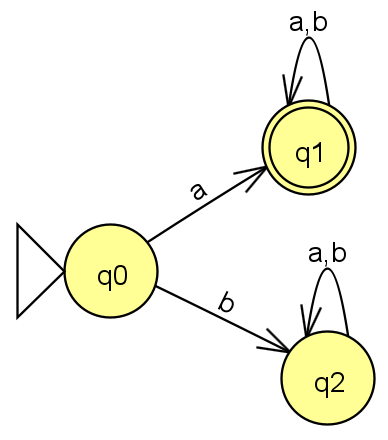
\includegraphics[width=0.2\textwidth]{../../../images/DFAs/ex1_q1.png}



% \vspace{3cm}
% \begin{flushleft}
% أرجو لكم وقتًا ممتعًا.

% الأستاذ محمود اغبارية.
% \end{flushleft}


% \end{document}


\title{وظيفة بيتية 5 للصف العاشر 10 \\ عمليات خارجية}
\begin{document}

\maketitle
\thispagestyle{fancy}

\begin{boxCode}
    \begin{itemize}
        \item كل سؤال يتطلب تعريف عملية خارجية واستدعاءها في الدالة \textenglish{Main}.
        \item إذا كانت العملية ترجع قيمة معينة، عليك طباعة هذه القيمة في العملية الرئيسية \textenglish{Main}.
        \item احرص على أن تكون أنواع المعطيات والترجيع مطابقة لما هو مطلوب في السؤال.
        \item \textbf{تذكّر:} "تتلقى" أي تأخذ القيمة في برامتر. أمّا "تستقبل" أي تقرأ القيمة من المستخدم.
    \end{itemize}
\end{boxCode}

\ifwithsols
\begin{enumerate}[itemsep=3em]
\else
\begin{enumerate}
\fi

\item
اكتب عملية خارجية \textbf{تتلقى عددًا صحيحًا} وتميّز ما إذا كان العدد \textbf{زوجيًا أم فرديًا}. \\
تطبع \textenglish{"Even"} إذا كان زوجيًا و \textenglish{"Odd"} إذا كان فرديًا.
لا تعيد العملية أي قيمة.

\ifwithsols
\begin{boxSolution}
\begin{english}
\begin{minted}{csharp}
public static void PrintEvenOdd(int n)
{
    if (n % 2 == 0)
    {
        Console.WriteLine("Even");
    }
    else
    {
        Console.WriteLine("Odd");
    }
}

public static void Main()
{
    int n = int.Parse(Console.ReadLine());
    PrintEvenOdd(n);
}
\end{minted}
\end{english}
\end{boxSolution}
\clearpage
\fi


\item
اكتب عملية خارجية \textbf{تتلقى عددًا عشريًا} وتُعيد \textenglish{true} إذا كان العدد أكبر من صفر،
و\textenglish{false} إذا كان سالبًا أو صفرًا.

\ifwithsols
\begin{boxSolution}
\begin{english}
\begin{minted}{csharp}
public static bool IsPositive(double x)
{
    return x > 0;
}

public static void Main()
{
    double x = double.Parse(Console.ReadLine());
    Console.WriteLine(IsPositive(x));
}
\end{minted}
\end{english}
\end{boxSolution}
\fi


\item
اكتب عملية خارجية \textbf{تتلقى عددين صحيحين} وتُعيد الفرق المطلق بينهما
ثم استدعها واطبع الناتج.

\ifwithsols
\begin{boxSolution}
\begin{english}
\begin{minted}{csharp}
public static int AbsDiff(int a, int b)
{
    return Math.Abs(a - b);
}

public static void Main()
{
    int a = int.Parse(Console.ReadLine());
    int b = int.Parse(Console.ReadLine());
    Console.WriteLine(AbsDiff(a, b));
}
\end{minted}
\end{english}
\end{boxSolution}
\clearpage
\fi

\item
\begin{enumerate}
    \item أكتب عملية خارجية تتلقى 3 أعداد صحيحة، على العملية أن تفحص إن كان هناك عددان مجموعهما يساوي 100 وتطبع كلمة \textenglish{"Yes"}، خلاف ذلك تطبع \textenglish{"No"}.
    \item قم باستدعاء العملية من قسم أ مع الأعداد \textenglish{50, 30, 70}.
    \item قم باستدعاء العملية من قسم أ مع أعداد كما تشاء بشرط أن تكون نتيجة الطباعة \textenglish{"No"}.
    \item أكتب مقطع برنامج يستقبل 3 أعداد صحيحة، وعلى البرنامج أن يفحص إن كان هناك عددان مجموعهما يساوي 100 ويطبع جملة ملائمة. ملاحظة: عليك الاستعانة بالعملية من بند أ.
\end{enumerate}

\ifwithsols
\begin{boxSolution}
\begin{english}
\begin{minted}{csharp}
public static bool DoesPairSumTo100(int a, int b, int c)
{
    if( (a + b == 100) || (a + c == 100) || (b + c == 100) )
    {
        return true;
    }
    else
    {
        return false;
    }
}

public static void Main()
{
    // b.
    bool result = DoesPairSumTo100(50, 30, 70);
    Console.WriteLine(result);

    // c.
    result = DoesPairSumTo100(60, 30, 90);
    Console.WriteLine(result);

    // d.
    int a = int.Parse(Console.ReadLine());
    int b = int.Parse(Console.ReadLine());
    int c = int.Parse(Console.ReadLine());
    result = DoesPairSumTo100(a, b, c);
    Console.WriteLine(result);
}
\end{minted}
\end{english}
\end{boxSolution}
\clearpage
\fi

\clearpage
\item
\begin{enumerate}
\item أكتب عملية خارجية تتلقى عددين صحيحين، على العملية أن تفحص إن كان أحد العددين ضعف الآخر تمامًا (أي $a = 2 \times b$ أو $b = 2 \times a$)، وتطبع \textenglish{"Double"} إذا تحقق الشرط، وإلا تطبع \textenglish{"Not Double"}.
\item قم باستدعاء العملية من قسم أ مع الأعداد \textenglish{4, 2}.
\item قم باستدعاء العملية من قسم أ مع أعداد كما تشاء بشرط أن تكون نتيجة الطباعة \textenglish{"Not Double"}.
\item أكتب مقطع برنامج يستقبل عددين عشريين ويفحص إذا كان أحدهما ضعف الآخر، باستخدام العملية من بند أ.
\end{enumerate}
\ifwithsols
\begin{boxSolution}
\begin{english}
\begin{minted}{csharp}
public static void PrintDoubleOrNot(int a, int b)
{
    if (a == 2*b || b == 2*a)
    {
        Console.WriteLine("Double");
    }
    else
    {
        Console.WriteLine("Not Double");
    }
}

public static void Main()
{
    // b) example
    PrintDoubleOrNot(4, 2);
    // c) another example
    PrintDoubleOrNot(5, 3);
    // d) read and check
    int x = int.Parse(Console.ReadLine());
    int y = int.Parse(Console.ReadLine());
    PrintDoubleOrNot(x, y);
}
\end{minted}
\end{english}
\end{boxSolution}
\clearpage
\fi

\item
\begin{enumerate}
    \item أكتب عملية خارجية تتلقى 3 أعداد صحيحة، وتفحص إن كانت الأعداد مرتّبة تصاعديًا (كل عدد أكبر من السابق).
    تطبع \textenglish{"Ascending"} إذا كان الشرط صحيحًا، وإلا تطبع \textenglish{"Not Ascending"}.
    \item قم باستدعاء العملية من قسم أ مع الأعداد \textenglish{3, 7, 10}.
    \item قم باستدعاء العملية من قسم أ مع أعداد كما تشاء بحيث تكون النتيجة \textenglish{"Not Ascending"}.
    \item أكتب مقطع برنامج يستقبل 3 أعداد صحيحة ويفحص إن كانت مرتبة تصاعديًا بالاستعانة بالعملية من بند أ.
\end{enumerate}
\ifwithsols
\begin{boxSolution}
\begin{english}
\begin{minted}{csharp}
public static void PrintAscending(int a, int b, int c)
{
    if (a < b && b < c)
    {
        Console.WriteLine("Ascending");
    }
    else
    {
        Console.WriteLine("Not Ascending");
    }
}

public static void Main()
{
    // b) example
    PrintAscending(3, 7, 10);
    // c) another example
    PrintAscending(5, 3, 9);
    // d) read and check
    int x = int.Parse(Console.ReadLine());
    int y = int.Parse(Console.ReadLine());
    int z = int.Parse(Console.ReadLine());
    PrintAscending(x, y, z);
}
\end{minted}
\end{english}
\end{boxSolution}
\clearpage
\fi

% \item
% \begin{enumerate}

% \item أكتب عملية خارجية تتلقى 3 أعداد صحيحة، وتفحص إن كانت تشكّل أضلاع مثلث قائم الزاوية (أي يتحقق قانون فيثاغورس $a^2 + b^2 = c^2$ لأي ترتيب بين الأضلاع).
% تطبع \textenglish{"Right"} إذا كانت الأضلاع تشكل مثلثًا قائمًا، و \textenglish{"Not Right"} خلاف ذلك.
% \item قم باستدعاء العملية من قسم أ مع الأعداد \textenglish{3, 4, 5}.
% \item قم باستدعاء العملية من قسم أ مع أعداد أخرى بحيث تكون النتيجة \textenglish{"Not Right"}.
% \item أكتب مقطع برنامج يستقبل 3 أعداد صحيحة، ويفحص إن كانت تشكل مثلثًا قائمًا بالاعتماد على العملية من بند أ.
% \end{enumerate}

\end{enumerate}


\vspace{1cm}
\begin{flushleft}
أرجو لكم وقتًا ممتعًا.

الأستاذ محمود اغبارية.
\end{flushleft}


\end{document}
